\section{Вступ}
	
	Завершення знаходження всіх частинок Стандартної Моделі (SM) з відкриттям бозона Хіггса, і досягнень у космології  появляться необхідність вивчення та розуміння фізики за межами Стандартної Моделі (BSM). Але експерименти та фізичні теорії на цей час не задають конкретних напрямків для пошуку цієї нової фізики.
			
	Протягом наступних десятиліть існуючі масові рамки фізики будуть всебічно досліджуватися на таких експериментах як ATLAS, CMS, LHCb, Belle2 та NA62 \cite{NA62_TDR}. В той же час багатьма теоретичними моделями, що закривають недоліки СМ, передбачають існування так званих прихованиї частинок, що взаємодіють з частинками SM дуже слабо. Таким чином велика частина фізики в області доступних енергій досі залишається невивченою і відкрита для досліджень.
	
	В такій ситуації SHiP це нещодавно анонсований експеримент з фіксованою мішенню на прискорювачі SPS (CERN) націлений на вивчення 	області фізики прихованих частинок, а також на вивчення нейтринної фізики(в особливості $\tau$ нейтрино. Приховані частинки передбачаються багатьма моделями поза СМ. Інтенсивний пучок 400 GeV від SPS дозволяє дослідження багатьох моделей, які допускають існування легких екзотичних частинок з масою нижче 10 $GeV/c^2$ та великим часом життя, включаючи слабовзаємодіючі низькоенергетичні суперсиметричні(SUSY) стани.	
		
	\subsection{Огляд експерименту}
	
	На енергіях доступних на прискорювачі SPS приховані частинки в основному утворюються в результаті розпаду адронів, частково в розпадах зачарованих та красивих адронів вище маси каона.

	\begin{figure}[!h]
	\centering
	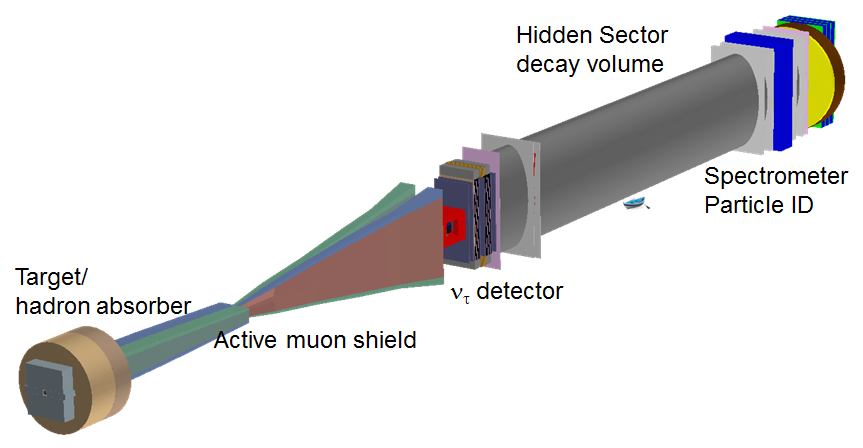
\includegraphics[width=0.9\textwidth]{introduction/SHiP-facility-overview}
	\caption{Експериментальна установка SHiP \cite{ship_TP}. }
	\label{fig:detector-overwiew}
	\end{figure}
	
	Детектор для прямого детектування прихованих частинок спроектований на повну реконструкцію цих ексклюзивних розпадів. Табл.\ref{table:req_decaymodes} узагальнює головні канали розпаду прихованих частинок в різноманітних фізичних моделях.
	
	
	\begin{table}[htb]
\begin{center}
\caption{ Головні канали розпаду прихованих частинок в різноманітних теоріях ($\ell = e, \mu$).}
\label{table:req_decaymodes}
\vspace{2mm}
\begin{tabular}{ll}
\hline
Модель	& Продукти розпаду \\
\hline
Neutrino portal, SUSY neutralino                 & $\ell^{\pm}\pi^{\mp}, \ell^{\pm} K^{\mp}, \ell^{\pm}\rho^{\mp},\,\,\,\,\, \rho^{\pm}\rightarrow \pi^{\pm}\pi^0$ \\
Vector, scalar, axion portals, SUSY sgoldstino   & $\ell^+\ell^-$ \\
Vector, scalar, axion portals, SUSY sgoldstino   & $\pi^+\pi^-, K^+K^-$ \\
Neutrino portal ,SUSY neutralino, axino          & $\ell^+\ell^-\nu$ \\
Axion portal, SUSY sgoldstino                    & $\gamma\gamma$ \\
% Axino ?                                          & $\gamma$... \\ 
SUSY sgoldstino                                  & $\pi^0\pi^0$ \\
\hline
\end{tabular}
\end{center}
\end{table}

	Принциповий фон при детектуванні прихованих частинок виникає від непружних розсіянь нейтрино і моюнів в об’ємі детектора, що  утворють довгоживучі частинки.
	
	Пучок же при постановці експерименту проектується так, щоб мінімізувати це фонове джерело частинок. Протон, при взаємодії з мішенню призводить до рясного утворення короткоживучих резонансів, піонів і каонів. В той час як для гальмування адронів достатньо декількох метрів заліза мішені, на виході з мішені маємо великий потік електромагнітного випромінювання утвореного в мішені, продуктів розпаду піонів, каонів і короткоживучих  резонансів утворених в мішені. Більшою частиною це є мюони і нейтрино. Для зменшення потоку нейтрино, зокрема потоку мюонних нейтрино і асоційованих мюонів, піони і кони необхідно зупинити якомога ефективніше ще до їх розпаду. Таким чином мішень має бути зроблена з матеріалу з найменшою довжиною взаємодії і бути достатньо довгою щоб комплексно вмістити адронну зливу по всіх напрямках поширення. Так як кути розльоту прихованих частинок очікуються достатньо великими, то жорстких вимог до розмірів до поперечного розміру пучка немає.
	
%	The principal background to the hidden particle decay signal originates from the inelastic scattering of neutrinos and muons in the vicinity of the detector producing long-lived particles.
	
%	The beam line is designed to minimize the background sources. The proton interaction in the target gives rise to a copious direct production of short-lived resonances, and pions and kaons. While a hadron stopper of a few metres of iron is sufficient to absorb the hadrons and the electromagnetic radiation emerging from the target, the decays of pions, kaons and short-lived resonances result in a large flux of muons and neutrinos. 	In order to reduce the flux of neutrinos, in particular the flux of muon neutrinos and the associated muons, the pions and kaons should be stopped as efficiently as possible before they decay. The target must therefore be made of a material with the shortest possible interaction length and be sufficiently long to contain the hadronic showers with minimum leakage. Since the production angle of the  hidden particles is relatively large, there is no requirement to minimize the beam spot.

	Корткоживучі резонанси і залишковий потік піонів і каонів після розпаду все ще  продукують інтенсивний потік мюонів. Цього потоку потрібно позбутися для запобігання потрапляння його в довірчий об'єм детектора або пасивним щитом або за допомогою активного щита на основі магнітного відхилення. В свою чергу це залишковий потік має бути достатньо низьким, щоб не перевищувати сприйнятливість $\tau$ нейтрино детектора. Як зображено на  Рис.\ref{fig:detector-overwiew}, для цієї цілі в основу детектора покладено 48м у довжину і 5м в ширину мюонний щит заснований на принципі магнітного відхилення мюонів в горизонтальній площині.

%	The short-lived resonances and the residual flux of decaying pions and kaons still give rise to a large flux of muons. This flux must be efficiently cleared from the detector fiducial volume by either a passive shield or through an active shield based on magnetic deflection. The residual flux should also be low enough so not to compromise the occupancy limit in the tau neutrino detector. As illustrated in Figure \ref{fig:detector-overwiew}, in the baseline design a 5 m horizontally wide region respecting these requirements has been achieved with a 48 m long active muon shield based on magnetic deflection of the muons in the horizontal plane.
	 
	Одразу після мюонного щита розташований 10м у довжину детектор $\tau$ нейтрино, після якого починається сектор для розпаду прихованих частинок (HS decay volume) 64м у довжину \cite{ship_TP}. Основна ціль тау нейтрино детектора  -- здійснити пряме спостереження $\overline{\nu}_\tau$, а також вивчити переріз взаємодії $\nu^\tau$ і $\overline{\nu}_\tau$.
	 
	На сьогоднішній день виходячи з розмірів мюонного щита і вартості детектора  сектор розпаду HS має еліптичний переріз з 5м в ширину в 10м у висоту. Довжина танкера вибиралася з міркувань вміщення подій розпаду прихованих частинок і кутових характеристик продуктів розпаду прихованих частинок.
	 
	 
%	The muon shield is followed by the 10 m long tau neutrino detector, which puts the start of the HS decay volume at about 64 m \cite{ship_TP}. The main purpose of the tau neutrino detector is to perform the first direct observation of the $\overline{\nu}_\tau$, and to study the properties and the cross section of $\nu^\tau$ and $\overline{\nu}_\tau$.
% The current optimization of muon shield and cost, results in a decay volume with an elliptical shape of 5 m width and 10 m height. The length of the decay volume is obtained by maximizing the acceptance to the hidden particle decay products given the transversal size.

	Для повної реконструкції подій розпаду прихованих частинок (ПЧ) необхідно мати магнітний спектрометр і систему ідентифікацію частинок в кінці об'єму розпаду. 

	Система ідентифікації розпаду частинок вимагає наявності електромагнітного калориметра для $e / \gamma$ ідентифікації з достатньою гранулярністю і роздільною здатністю по енергії для ефективної реконструкції $\pi^0$, а також наявності адронного калоримтра в комбінації з мюонним детектором для  $ \pi / \mu$ сепарації.
	
%	The full reconstruction of the hidden particle decays requires a magnetic spectrometer and a system for particle identification at the end of the decay volume.
	
%	The particle identification system requires an electromagnetic calorimeter for $e / \gamma$ identification with sufficient granularity and energy resolution in order to reconstruct $\pi^0$'s, and a hadron calorimeter in combination with a muon detector for $ \pi / \mu$ separation.
	
	\begin{figure}[!h]
	\centering
	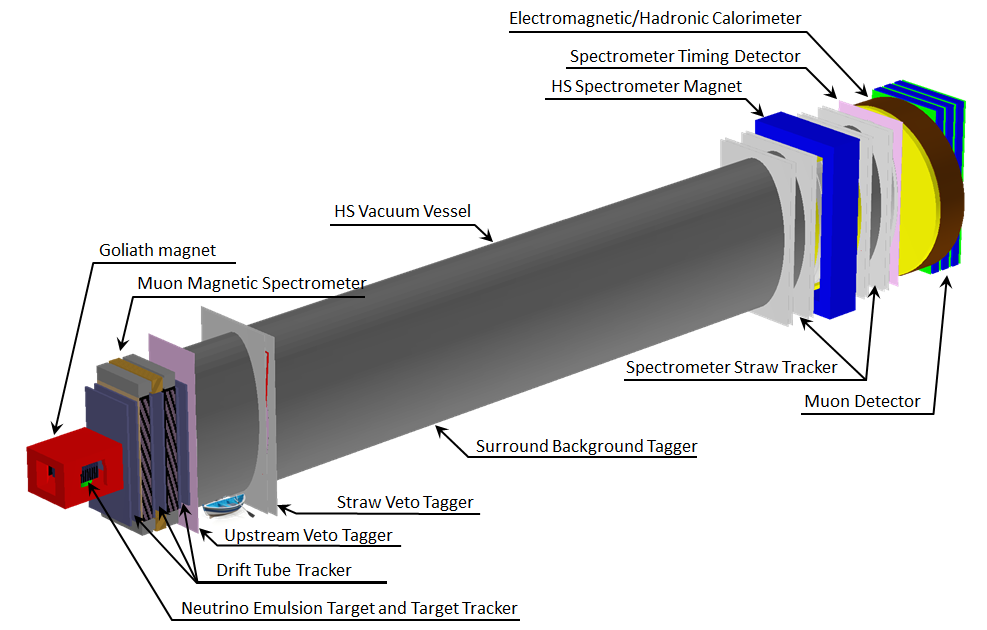
\includegraphics[width=\textwidth]{SHiP-detector-overview}
	\caption{SHiP детектор \cite{ship_TP}.}
	\end{figure}
	
	\subsection{Спектрометричний трекер в експерименті SHiP}
	
	Спектрометричний трекер є частиною системи ідентифікації типу частинок. Мета даного спектрометра -- реконструювати з високою ефективністю треки від заряджених частинок утворених в результаті розпаду прихованих частинок. Спектрометр повинен точно визначати імпульс частинки і траєкторію руху частинки. 
	
%	Spectrometer tracker is a part of particle identification system.  The purpose of the HS spectrometer is to reconstruct with high efficiency the tracks of charged particles from the decay of hidden particles. The spectrometer must provide an accurate determination of the track momentum and of the flight direction within the fiducial decay volume.
	
	\begin{figure}[!h]
		\centering
		\subfloat[ Розташування шарів трекера і дипольного магніту. Інтенсивність компоненти магнітного поля $B_x$ як функція від z.]{
			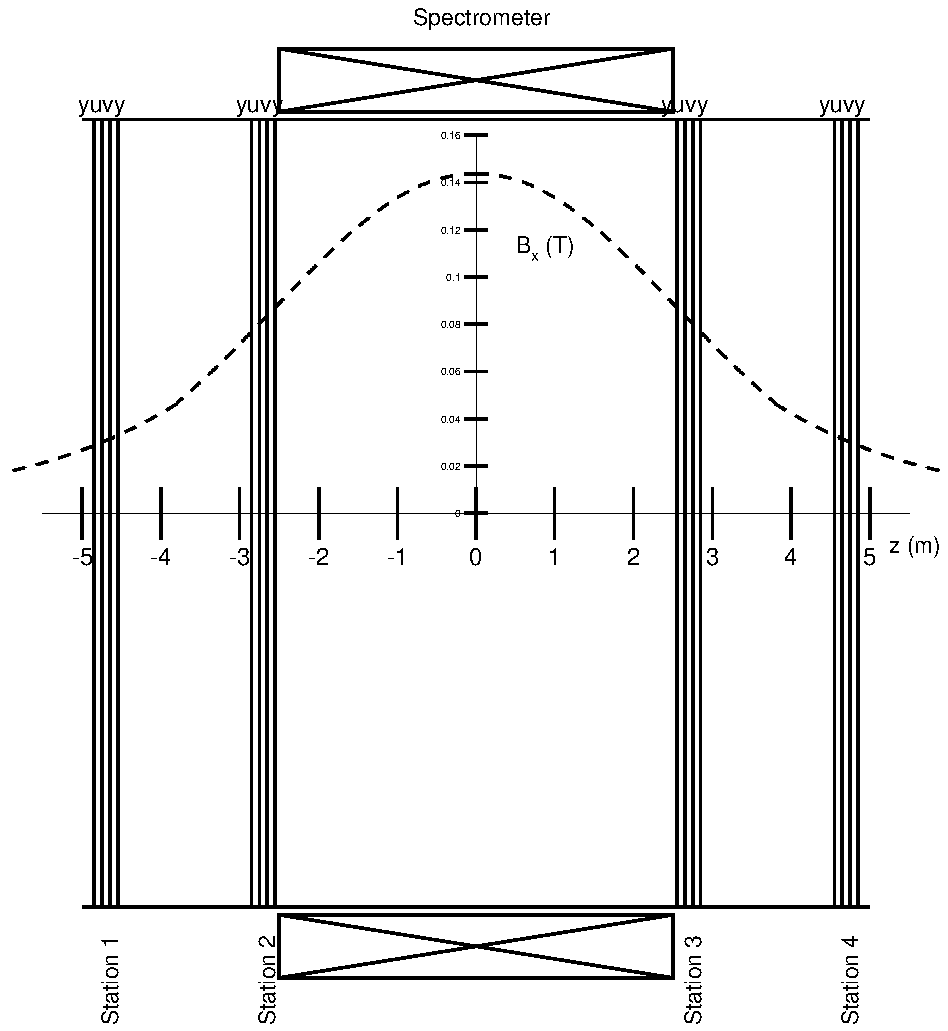
\includegraphics[width=0.4\textwidth]{introduction/spectrometer-layout} 
			\label{fig:spectrometer_layout} }%
		\qquad
		\subfloat[ Фронтальний вигляд на шари однієї секції трекера. Червоним кольором зображено довірча область реєстрації частинок(згідно до параметрів довірчого HS об'єму]{
			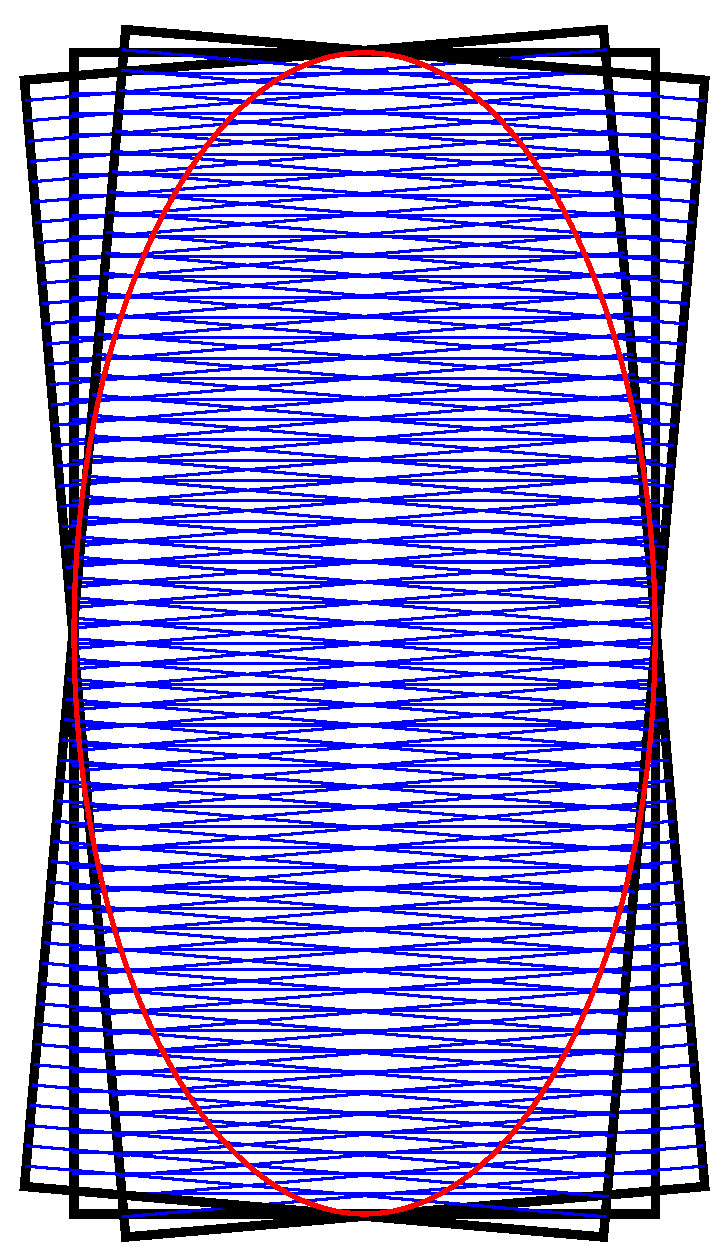
\includegraphics[width=0.4\textwidth]{introduction/straw-views.pdf} 
			\label{fig:cluster_distrib} }%
		\caption{Схема спектрометра}
	\end{figure}

	Спектрометр складається з весокоапертурного дипольного магніту і двох телескопів по обидві сторони від магніту. Схема з чотирма трековими системами симетрична відносно магніту і зображена на Рис.\ref{fig:spectrometer_layout}. Розмір дипольного магніту по горизонталі 5м, 10 по вертикалі і 5м у довжину. Такі параметри забезпечують гарне поле, необхідне для експерименту при прийнятній ціні.
	
%	The spectrometer consists of a large aperture dipole magnet and two tracking telescopes on each side of the magnet. A layout with four tracking stations symmetrically arranged around the dipole magnet, as depicted in Figure \ref{fig:spectrometer_layout}, is taken as a baseline. The size and layout of the tracker stations is connected to the size of the magnet. A dipole spectrometer magnet with a horizontal gap of 5 m, a height of 10 m and a length of 5 m provides good acceptance coverage and is considered feasible at a reasonable cost.

	Виходячи з напрямку магнітного поля дрейфові чутливі елементи(дрейфові трубки) розташовані горизонтально для точного вимірювання вертикальної (Y) координати. Два стерео шари (U і V) повернуті відносно горизонтального на кути $ \pm \theta _{stereo}$ відповідно для виміру поперечної координати Х з точністю $ \sim 1/ \sin \theta _{stereo}$. Точність по осі X (а заодно і значення стерео кута) визначається з  огляду на необхідність великої роздільної здатності для визначення  вершини розпаду і куту розльоту дочірніх частинок, що формують інваріантну масу. Кожна позиційно чутлива секція складається з чотирьох профілів(Y-U-V-Y) чутливих елементів. Дві секції по одну сторону від магніту розташовані на відстані $\bigtriangleup = 2 m$ одна від одної. Проміжок між секціями (2,3) "суміжними" до магніту рознесені на відстань 5м.

%	Following the direction of the magnetic field, the measuring elements are oriented horizontally to measure precisely the vertical (Y) coordinate. Two stereo views (U and V) are rotated by an angle $ \pm \theta _{stereo}$ for measuring the transverse coordinate X with an accuracy degraded by $ \sim 1/ \sin \theta _{stereo}$. 	The precision in X (i.e. the value of the stereo angle) is driven by the need of a good enough measurement of the decay vertex, opening angle of the daughter particles (which enters the invariant mass) and impact parameter at the production target. Each station contains 4 views (Y-U-V-Y). The two stations on the same side of the magnet are separated by $\bigtriangleup = 2 m$ and a gap of $5 m$ is left between the second and third stations (i.e. each is $2.5 m$ away from the centre of the magnet).

	Таким чином трекова частина магнітного спектрометра повинна забезпечувати хорошу просторову роздільну здатність, а також має мінімізувати вклад від багаторазового розсіяння. На додаток трекер має працювати у вакуумі. Трекер з дрейфових трубок виготовлених з тонкого поліетилентерефталату (ПЕТ) ідеально підходить для досягнення цих цілей. Газонепроникність цих труб була продемонстрована в довгострокових дослідженнях, і процедура масового виробництва також добре відома (див. екперимент NA62 \cite{NA62_TDR}). Головна принципова різниця в трубка необхідних для SHiP порівняно з NA62 це довжина трубок -- 5м порівняно з (2.1м в NA62). Таким чином основні зміни згідно предмету цікавості від SHiP (EoI \cite{EoI}) виливається у використання іншого спектрометричного магніту, також орієнтацією дрейфових трубок, а також збільшення поперечних розмірів детектору.
	
%	The tracking stations of the magnetic spectrometer must provide good spatial resolution and minimise the contribution from multiple scattering. In addition, the tracker must operate in vacuum. A straw tracker made of thin polyethylene terephthalate (PET) tubes is ideal to meet these goals. Gas tightness of these tubes has been demonstrated in long term tests and the mass production procedure is also well established (see NA62 experiment \cite{NA62_TDR}). The main differences between the SHiP tracker and the NA62 tracker are the need for $5 m$ long straws (vs 2.1 m in NA62). The main changes with respect to the Expression of Interest \cite{EoI} follow from the changes applied to the spectrometer magnet. The straw orientation has been turned from vertical to horizontal and one transverse dimension has been increased from 5 to 10 m.
	